\subsection{תיקון מסדר שני}
נחזור לפיתוח. נסתכל על $u_1=u(\Delta)$ בסדר גבוה יותר
$$u_1=u_0'\Delta + \frac{u''_0}{2}\Delta^2 + O(\Delta^3) = - \frac{u''_0\Delta}{2Z} + \frac{u''_0}{2}\Delta^2 = u''_0\left(\frac{Z\Delta^2-\Delta}{2Z}\right)$$
כלומר 
$$u''_0=\frac{2Z}{Z\Delta^2-\Delta}u_1\quad\Rightarrow\quad H^{(2)}_{11} = H_{11} + \frac{1}{12}\frac{Z}{Z\Delta^2-\Delta} $$
נשאר רק להסתכל על התוצאות. התיקון מסדר שני עובד בצורה טובה, אפילו טובה יותר ממה שציפיתי.
\begin{figure}[h!]
    \begin{minipage}[t]{0.45\textwidth}
        \centering
        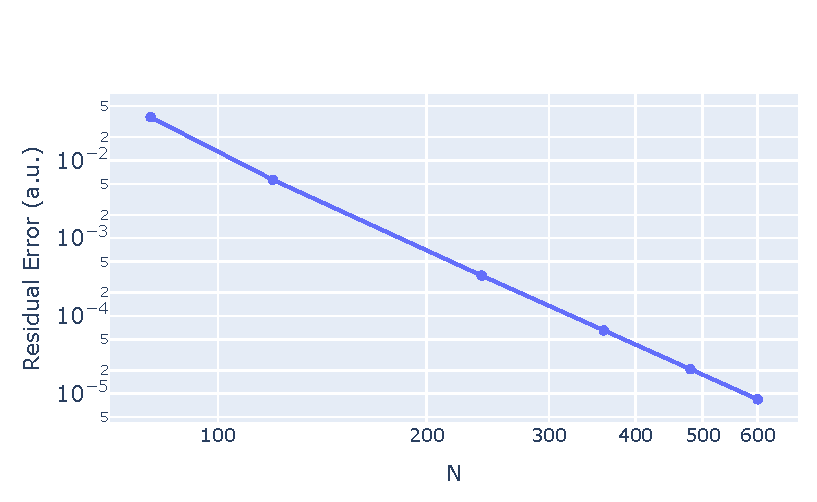
\includegraphics[width=\linewidth]{plots/second_order/residual_error.eps}
        \caption{השגיאה השיורית השוואה בין המצב ללא תיקון, תיקון מסדר ראשון ותיקון מסדר שני }
        \label{fig:second_order_residual_error}
    \end{minipage}
    \hfill
    \begin{minipage}[t]{0.45\textwidth}
        \vspace{-2cm}
        \centering
        \begin{tabular}{c c}
תיקון & $q$ \\
\hline
ללא תיקון & $1.5539$ \\
תיקון מסדר ראשון & $2.26972$ \\
תיקון מסדר שני & $4.56825$ \\
\end{tabular}

        \captionof{table}{קצב ההתכנסות עבור רמות התיקון השונות}
        \label{tab:second_order_convergence_rates}
    \end{minipage}
\end{figure}
